\documentclass[]{beamer}
\usetheme{Boadilla}
\usepackage{tikz}
\usetikzlibrary{positioning}
\usetikzlibrary{shapes.multipart}
%\usepackage{minted}
\usepackage{fancyvrb}
\usepackage[utf8]{inputenc}
\usepackage{graphicx}
\usepackage{xcolor}
\usepackage{listings}
\usepackage{tabulary}
\usepackage{colortbl}

\newcommand\warning{%
 \makebox[1.4em][c]{%
 \makebox[0pt][c]{\raisebox{.1em}{\scriptsize!}}%
 \makebox[0pt][c]{\color{red}\normalsize$\bigtriangleup$}}}%
		
%New colors defined below
\definecolor{codegreen}{rgb}{0,0.6,0}
\definecolor{codegray}{rgb}{0.5,0.5,0.5}
\definecolor{codepurple}{rgb}{0.58,0,0.82}
\definecolor{backcolour}{RGB}{240,240,240}

%Code listing style named "mystyle"
\lstdefinestyle{mystyle}{
  backgroundcolor=\color{backcolour},   commentstyle=\color{codegreen},
  keywordstyle=\color{blue},
  numberstyle=\tiny\color{codegray},
  stringstyle=\color{orange},
  basicstyle=\ttfamily\footnotesize,
  breakatwhitespace=false,         
  breaklines=true,                 
  captionpos=b,                    
  keepspaces=true,                 
  numbers=none,                    
  numbersep=5pt,                  
  showspaces=false,                
  showstringspaces=false,
  showtabs=false,                  
  tabsize=2
}
 
\lstset{style=mystyle}
   
\renewcommand{\vec}[1]{\boldsymbol{#1}}
\newcommand{\ques}{\textbf{\textcolor{red}{Question:  }}}
\newcommand{\questionssofar}{\begin{frame}\frametitle{Any questions?}\end{frame}}

\title[Transfer Learning \& Tokenization]{Chapter 9: \\ Transfer Learning \& Tokenization}
\author{Matthias Aßenmacher}
\date{January 13, 2021}

\begin{document}


\begin{frame}
	\titlepage
\end{frame}



\begin{frame}{Recap: Word vectors}
	\begin{figure}
		\centering
		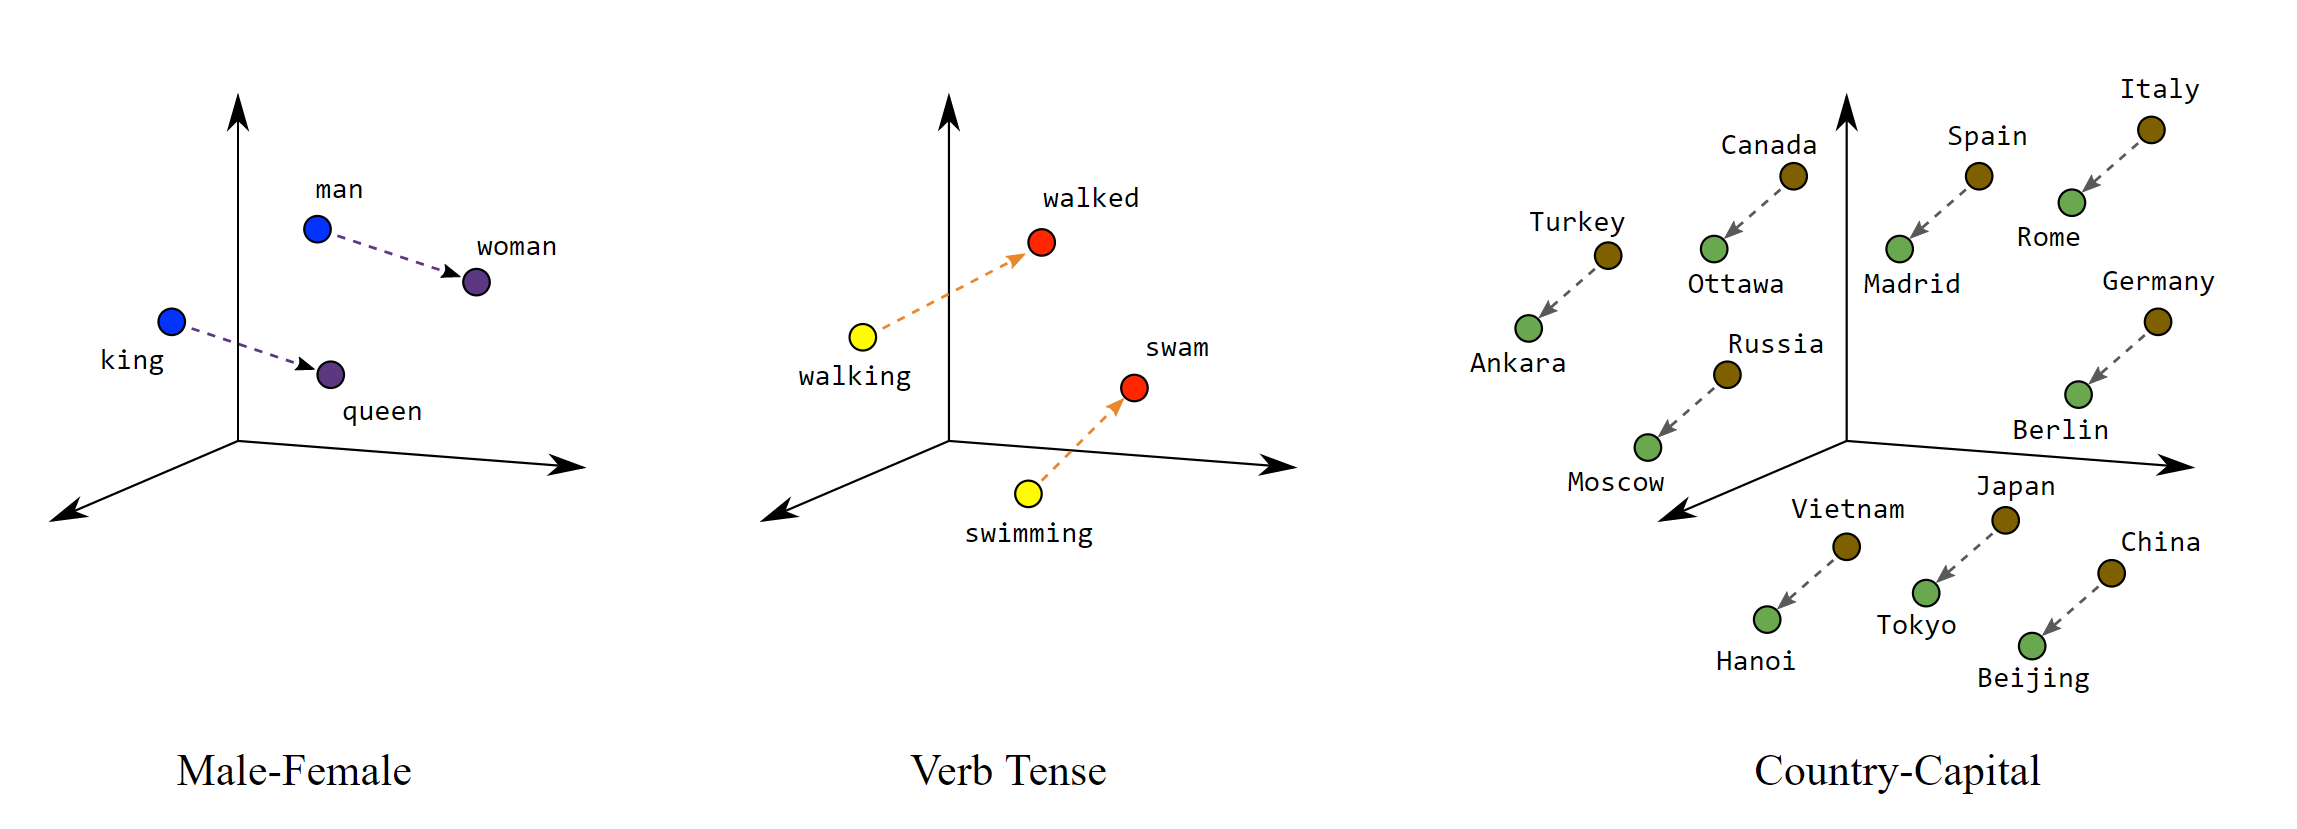
\includegraphics[width = 11cm]{figure/linear-relationships.png}\\ 
		\footnotesize{Source:} \href{https://developers.google.com/machine-learning/crash-course/embeddings/translating-to-a-lower-dimensional-space}{\footnotesize \it google}
	\end{figure}

	\begin{itemize}
		\item Information is encoded in (pre-)trained word embeddings
		\item Embeddings are used for tasks external to the training corpus
	\end{itemize}
\end{frame}



\begin{frame}{What is Transfer Learning?}

	\textbf{Wikipedia says:} \\
    \textit{"Transfer learning is a research problem in machine learning that focuses on storing knowledge gained while solving one problem and applying it to a different but related problem."}\\
		
	\vspace{.5cm}
	
	\textbf{How it works with word2vec}
	
	\begin{itemize}
		\item Train word2vec on some "fake task" (CBOW or Skip-gram)
		\item Extract the stored knowledge (a.k.a. embedding)\\
					\textit{or:} Directly download embeddings from the web 
		\item Perform a different (supervised) task using the embeddings
	\end{itemize}
\end{frame}



\begin{frame}{A remark on vocabulary \& tokenization}

	\textbf{Challenges:}

	\begin{itemize}
		\item If no embedding for a word exists, it cannot be represented.
		\item \textit{Workaround:}\\
			\begin{itemize}
				\item Train subword (character n-gram) embeddings
				\item Represent OOV word as combination of them
			\end{itemize}
		\item This is already a special case of \textbf{Tokenization}
	\end{itemize}
	
	\vspace{.3cm}
	
	\textbf{Tokenization examples:}
	
	\begin{itemize}
		\item Whitespace tokenization
		\item N-grams
		\item Character n-grams
		\item Characters
	\end{itemize}
\end{frame}



\begin{frame}{Fine-grained tokenization}

	\textbf{Difficulties:}

	\begin{itemize}
		\item When using embeddings (or other models/methods) for transferring knowledge, one has to stick to this method's tokenization scheme.
		\item Using words as tokens leads to vocabulary sizes of easily $> 100k$, which is undesirable.
		\item Characters as tokens lead to a very small vocabulary size but aggravate capturing meaning.
		\item Using (sets of) n-grams is kind of heuristic.
	\end{itemize}
	
	\vspace{.3cm}
	
	\textbf{Smart alternatives:}
	
	\begin{itemize}
		\item BytePair encoding \href{https://www.derczynski.com/papers/archive/BPE_Gage.pdf}{\beamergotobutton{Gage (1994)}} \href{https://www.aclweb.org/anthology/P16-1162.pdf}{\beamergotobutton{Sennrich et al. (2016)}}
		\item WordPiece \href{https://storage.googleapis.com/pub-tools-public-publication-data/pdf/37842.pdf}{\beamergotobutton{Schuster \& Nakajima (2012)}} \href{https://arxiv.org/pdf/1609.08144.pdf}{\beamergotobutton{Wu et al. (2016)}}
		\item SentencePiece \href{https://arxiv.org/pdf/1808.06226.pdf}{\beamergotobutton{Kudo et al. (2018)}}
	\end{itemize}
\end{frame}



\begin{frame}{BytePair encoding (BPE)}

	\textbf{Data compression algorithm \href{https://www.derczynski.com/papers/archive/BPE_Gage.pdf}{\beamergotobutton{Gage (1994)}}}

	\begin{itemize}
		\item Considering data on a \textit{byte}-level
		\item Looking at pairs of bytes:
			\begin{enumerate}
				\item Count the occurrences of all byte pairs
				\item Find the most frequent byte pair
				\item Replace it with an unused byte
			\end{enumerate}
		\item Repeat this process until no further compression is possible
	\end{itemize}
	
	\vspace{.3cm}
	
	\textbf{Open-vocabulary neural machine translation \href{https://www.aclweb.org/anthology/P16-1162.pdf}{\beamergotobutton{Sennrich et al. (2016)}}}
	
	\begin{itemize}
		\item Translation as an open-vocabulary problem
		\item Word-level NMT models:
			\begin{itemize}
				\item Handling out-of-vocabulary word by using back-off dictionaries
				\item Unable to translate or generate previously unseen words
			\end{itemize}
		\item Subword-level models alleviate this problem
	\end{itemize}
\end{frame}



\begin{frame}{BytePair encoding (BPE)}

	\textbf{Adapt BPE for word segmentation \href{https://www.aclweb.org/anthology/P16-1162.pdf}{\beamergotobutton{Sennrich et al. (2016)}}}

	\begin{itemize}
		\item \textit{Goal:} Represent an open vocabulary by a vocabulary of fixed size\\
					$\rightarrow$ Use variable-length character sequences 
		\item Looking at pairs of characters:
			\begin{enumerate}
				\item Initialize the the vocabulary with all characters plus end-of-word token
				\item Count occurrences and find the most frequent character pair,\\
							e.g. "A" and "B" (\warning Word boundaries are \textbf{not} crossed)
				\item Replace it with the new token "AB"
			\end{enumerate}
		\item Only one hyperparameter: Vocabulary size\\
					(Initial vocabulary + Specified no. of merge operations)\\
					$\rightarrow$ Repeat this process until given $|V|$ is reached
	\end{itemize}
\end{frame}



\begin{frame}{WordPiece}

	\textbf{Voice Search for Japanese and Korean \href{https://storage.googleapis.com/pub-tools-public-publication-data/pdf/37842.pdf}{\beamergotobutton{Schuster \& Nakajima (2012)}}}

	\begin{itemize}
		\item \textit{Specific Problems:} 
			\begin{itemize}
				\item Asian languages have larger basic character inventories compared to Western languages
				\item Concept of spaces between words does (partly) not exist
				\item Many different pronounciations for each character
			\end{itemize}
		\item \textit{WordPieceModel:} Data-dependent + do not produce OOVs
			\begin{enumerate}
				\item Initialize the the vocabulary with basic Unicode characters (22k for Japanese, 11k for Korean)\\
							\warning Spaces are indicated by an underscore attached before (of after) the respective basic unit or word (increases initial $|V|$ by up to factor 4)
				\item Build a language model using this vocabulary
				\item Merge word units that increase the likelihood on the training data the most, when added to the model
			\end{enumerate}
		\item Two possible stopping criteria:\\Vocabulary size \textit{or} incremental increase of the likelihood
	\end{itemize}
\end{frame}



\begin{frame}{WordPiece}

	\textbf{Use for neural machine translation \href{https://arxiv.org/pdf/1609.08144.pdf}{\beamergotobutton{Wu et al. (2016)}}}

	\begin{itemize}
		\item \textit{Adaptions:} 
			\begin{itemize}
				\item Application to Western languages leads to a lower number of basic units ($\sim$ 500)
				\item Add space markers (underscores) \textit{only} at the beginning of words
				\item Final vocabulary sizes between 8k and 32k yield a good balance between accuracy and fast decoding speed\\(compared to around 200k from \href{https://storage.googleapis.com/pub-tools-public-publication-data/pdf/37842.pdf}{\beamergotobutton{Schuster \& Nakajima (2012)}})
			\end{itemize}
	\end{itemize}
	
	\vspace{.3cm}
	
	\textit{Independent} \textbf{vs.} \textit{joint} \textbf{encodings for source \& target language}
	
	\begin{itemize}
		\item Sennrich et al. (2016) report better results for joint BPE
		\item Wu et al. (2016) use shared WordPieceModel to guarantee identical segmentation in source \& target language in order to facilitate copying rare entity names or numbers
	\end{itemize}
\end{frame}



\begin{frame}{SentencePiece \href{https://www.aclweb.org/anthology/D18-2012.pdf}{\beamergotobutton{Kudo et al. (2018b)}}}

	\textbf{No need for Pre-Tokenization}

	\begin{itemize}
		\item BPE \& WordPiece require a sequence of words as inputs\\
					$\rightarrow$ Some sort of (whitespace) tokenization has to be performed before their application
		\item SentencePiece (as the name already reveals) doesn't need that\\
					$\rightarrow$ Can be applied to "raw" sentences\\
					$\rightarrow$ Consists of \textit{Normalizer}, \textit{Trainer}, \textit{Encoder} \& \textit{Decoder}\\
					$\rightarrow$ Under the hood, two different algorithms are implemented
					\begin{itemize}
						\item byte-pair encoding \href{https://www.aclweb.org/anthology/P16-1162.pdf}{\beamergotobutton{Sennrich et al. (2016)}}
						\item unigram language model \href{https://www.aclweb.org/anthology/P18-1007.pdf}{\beamergotobutton{Kudo et al. (2018a)}}
					\end{itemize}
		\item No language-specific pre-processing
	\end{itemize}
	
	\vspace{.3cm}
	
	$\Rightarrow$ Basically a nice, end-to-end usable system/pipeline
	
\end{frame}



\begin{frame}{Back to Transfer Learning}

	\textbf{Embedding Idea + more complex architectures:}

	\begin{itemize}
		\item \textit{Naive approach:}\\
					Standard embeddings (like word2vec) are "\textit{context-free}"
		\item \textit{Better:}\\
			\begin{itemize}
				\item More complex networks, where the embeddings are trainable parameters of the model
				\item Model learns \textit{context sensitive} embeddings 
				\item We already encountered this in the Transformer
			\end{itemize}
		\item \textit{More complex networks:}\\
			\begin{itemize}
				\item Whole network just to learn the embeddings, \textit{or}
				\item Additional embedding-layer as the lowest layer
			\end{itemize}
	\end{itemize}
\end{frame}



\begin{frame}{Contextuality}

	\textbf{1st Generation of neural embeddings are "context-free":}

	\begin{itemize}
		\item Breakthrough paper by Mikolov et al, 2013 (Word2Vec)
		\item Followed by Pennington et al, 2014 (GloVe)
		\item Extension of Word2Vec by Bojanowski et al, 2016 (FastText)
	\end{itemize}
	
	\vspace{.3cm}
	
	\textbf{Why "Context-free"?}
	
	\begin{itemize}
		\item Models learn \textit{one single} embedding for each word
		\item Why could this possibly be problematic?
			\begin{itemize}
				\item "The \textit{default} setting of the function is xyz."
				\item "The probability of \textit{default} is rather high."
			\end{itemize}
		\item Would be nice to have different embeddings for these two occurrences
	\end{itemize}
\end{frame}



\begin{frame}{Transfer Learning -- Further Motivation}

	\textbf{Questions/Problems:}

	\begin{itemize}
		\item Where in this (deep) model do we achieve contextuality?\\
					(For sure \textit{not} in the lowest layer!)\\
					$\rightarrow$ Not straightforward to extract them
		\item The deeper the network ..  \\
			\begin{itemize}
				\item .. the more expensive to train
				\item .. the more data we need 
			\end{itemize}
					$\rightarrow$ You cannot just train them at home
	\end{itemize}
\end{frame}



\begin{frame}{Transfer Learning}

	\textbf{TRANSFER LEARNING}

	\begin{itemize}
		\item Train such an architecture on ..
			\begin{itemize}
				\item .. a fairly \textit{general} task
				\item .. which does not require any labels ("\textit{self-supervised}")
				\item .. using \textit{large} amounts of data
			\end{itemize}\mbox{}
		\item Do not extract static embeddings, but use the whole \textbf{\textit{pre-trained architecture}}\\\mbox{}
		\item Replace the final layer used for the \textit{general} task by a different layer for a \textit{specific} task at hand
	\end{itemize}
\end{frame}



\begin{frame}{Taxonomy of transfer learning \href{https://ruder.io/thesis/}{\beamergotobutton{Ruder, 2019}}}
	\begin{figure}
		\centering
		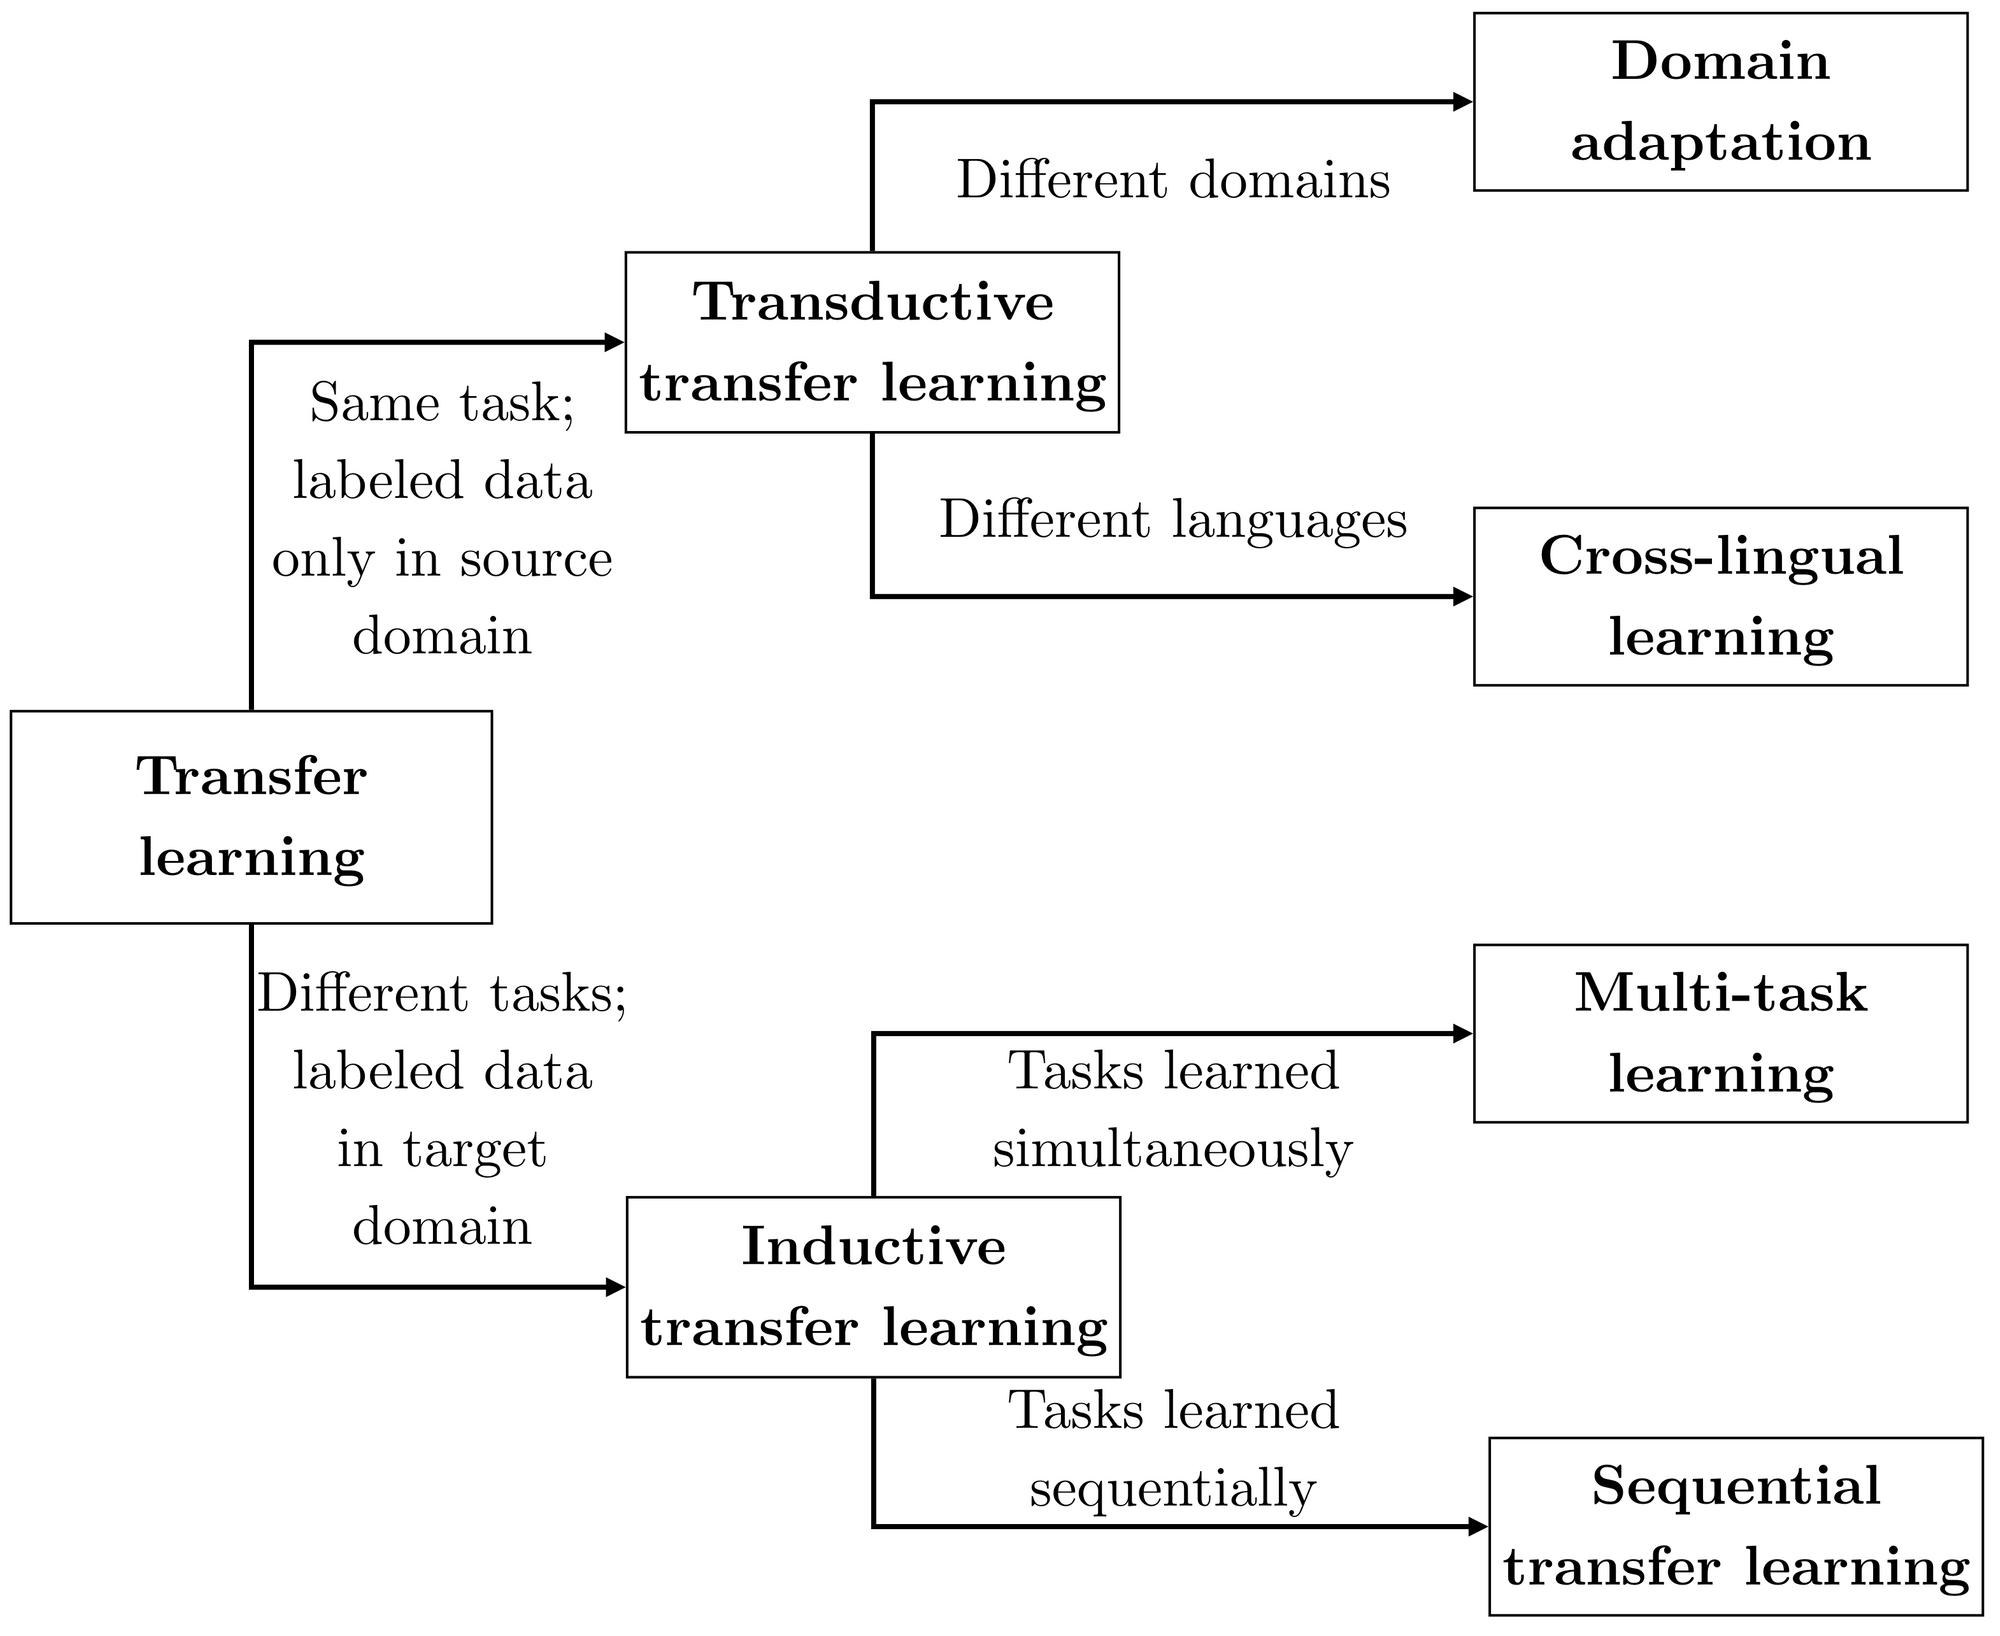
\includegraphics[width = 8cm]{figure/transfer_learning_taxonomy-1.png}\\ 
		\footnotesize{Source:} \href{https://ruder.io/thesis/}{\footnotesize \it Sebastian Ruder}
	\end{figure}
\end{frame}



\begin{frame}{Taxonomy of transfer learning \href{https://ruder.io/thesis/}{\beamergotobutton{Ruder, 2019}}}

	\textbf{Transductive Transfer learning}

	\begin{itemize}
		\item Domain adaptation:\\
					$\rightarrow$ "\textit{Transfer knowledge learned from performing task A on labeled data from domain X to performing task A in domain Y.}"\\\mbox{}
		\item Cross-lingual learning:\\
					$\rightarrow$ "\textit{Transfer knowledge learned from performing task A on labeled data from language X to performing task A in language Y.}"\\\mbox{}
		\item \textit{Important:} No labeled data in target domain/language \textit{Y}.
	\end{itemize}
\end{frame}



\begin{frame}{Taxonomy of transfer learning \href{https://ruder.io/thesis/}{\beamergotobutton{Ruder, 2019}}}

	\textbf{Inductive Transfer learning}

	\begin{itemize}
		\item Multi-task learning:\\
					$\rightarrow$ "\textit{Transfer knowledge learned from performing task A on data from domain X to performing multiple (simultaneous) tasks B, C, D, .. in domain Y.}"\\\mbox{}
		\item Sequential transfer learning:\\
					$\rightarrow$ "\textit{Transfer knowledge learned from performing task A on data from domain X to performing multiple (sequential) tasks B, C, D, .. in domain Y.}"\\\mbox{}
		\item \textit{Important:} Labeled data only for task(s) from target domain \textit{Y}.
	\end{itemize}
\end{frame}



\begin{frame}{Feature-based transfer learning}

	\textbf{Again: Word Embeddings}

	\begin{itemize}
		\item The stored knowledge from the pre-trained model is extracted \textbf{as is} and is not further adapted to the actual domain/task of interest.
		\item \textit{Difficulties:}
			\begin{itemize}
				\item Source \& target domain/task might be pretty different
				\item No representations for domain-/task-specific words
				\item No contextualization
			\end{itemize}
	\end{itemize}

	\textbf{Enhancement:} \textit{\textbf{E}mbeddings from \textbf{L}anguage \textbf{Mo}dels (ELMo)}

	\begin{figure}
		\centering
		
\includegraphics[width = 3cm]{figure/elmo.jpg}
	\end{figure}
\end{frame}



\begin{frame}{ELMo \href{https://www.aclweb.org/anthology/N18-1202.pdf}{\beamergotobutton{Peters et al., 2018}}}
	\begin{itemize}
		\item Bidirectional language model (LM)
		\item Combines a forward LM $$p\left(t_{1}, t_{2}, \ldots, t_{N}\right)=\prod_{k=1}^{N} p\left(t_{k} | t_{1}, t_{2}, \ldots, t_{k-1}\right)$$
					and a backward LM $$p\left(t_{1}, t_{2}, \ldots, t_{N}\right)=\prod_{k=1}^{N} p\left(t_{k} | t_{k+1}, t_{k+2}, \ldots, t_{N}\right)$$
					to arrive at the following loglikelihood:
					$$\begin{array}{l}
\sum_{k=1}^{N}\left(\log p\left(t_{k} | t_{1}, \ldots, t_{k-1} ; \Theta_{x}, \overrightarrow{\Theta}_{L S T M}, \Theta_{s}\right)\right. \\
\quad\left. +\log p\left(t_{k} | t_{k+1}, \ldots, t_{N} ; \Theta_{x}, \overleftarrow{\Theta}_{L S T M}, \Theta_{s}\right)\right)
\end{array}$$
	\end{itemize}
\end{frame}



\begin{frame}{ELMo embeddings}
	\begin{itemize}
		\item Character-based (context-independent) token representations $$x_k^{LM}$$
		\item Two-layer biLSTM as main architecture:
			\begin{itemize}
				\item Two context-dependent token representations \textit{per layer}, i.e.
							$$\overrightarrow{\mathbf{h}}_{k, j}^{L M}\; \mbox{\&}\; \overleftarrow{\mathbf{h}}_{k, j}^{L M}\; \mbox{for the $k$-th token in the $j$-th layer.}$$
				\item Four context-dependent token representations in total: 
							$$\left\{\overrightarrow{\mathbf{h}}_{k, j}^{L M}, \overleftarrow{\mathbf{h}}_{k, j}^{L M} | j = 1, 2\right\}$$
			\end{itemize}
		\item Five representations per token in total:
					$$\begin{aligned}
R_{k} &=\left\{\mathbf{x}_{k}^{L M}, \overrightarrow{\mathbf{h}}_{k, j}^{L M}, \overleftarrow{\mathbf{h}}_{k, j}^{L M} | j=1, \ldots, L\right\} \\
&=\left\{\mathbf{h}_{k, j}^{L M} | j = 0, 1, 2\right\}
\end{aligned}$$
	\end{itemize}
\end{frame}



\begin{frame}{ELMo -- Graphical representation}
	\begin{figure}
		\centering
		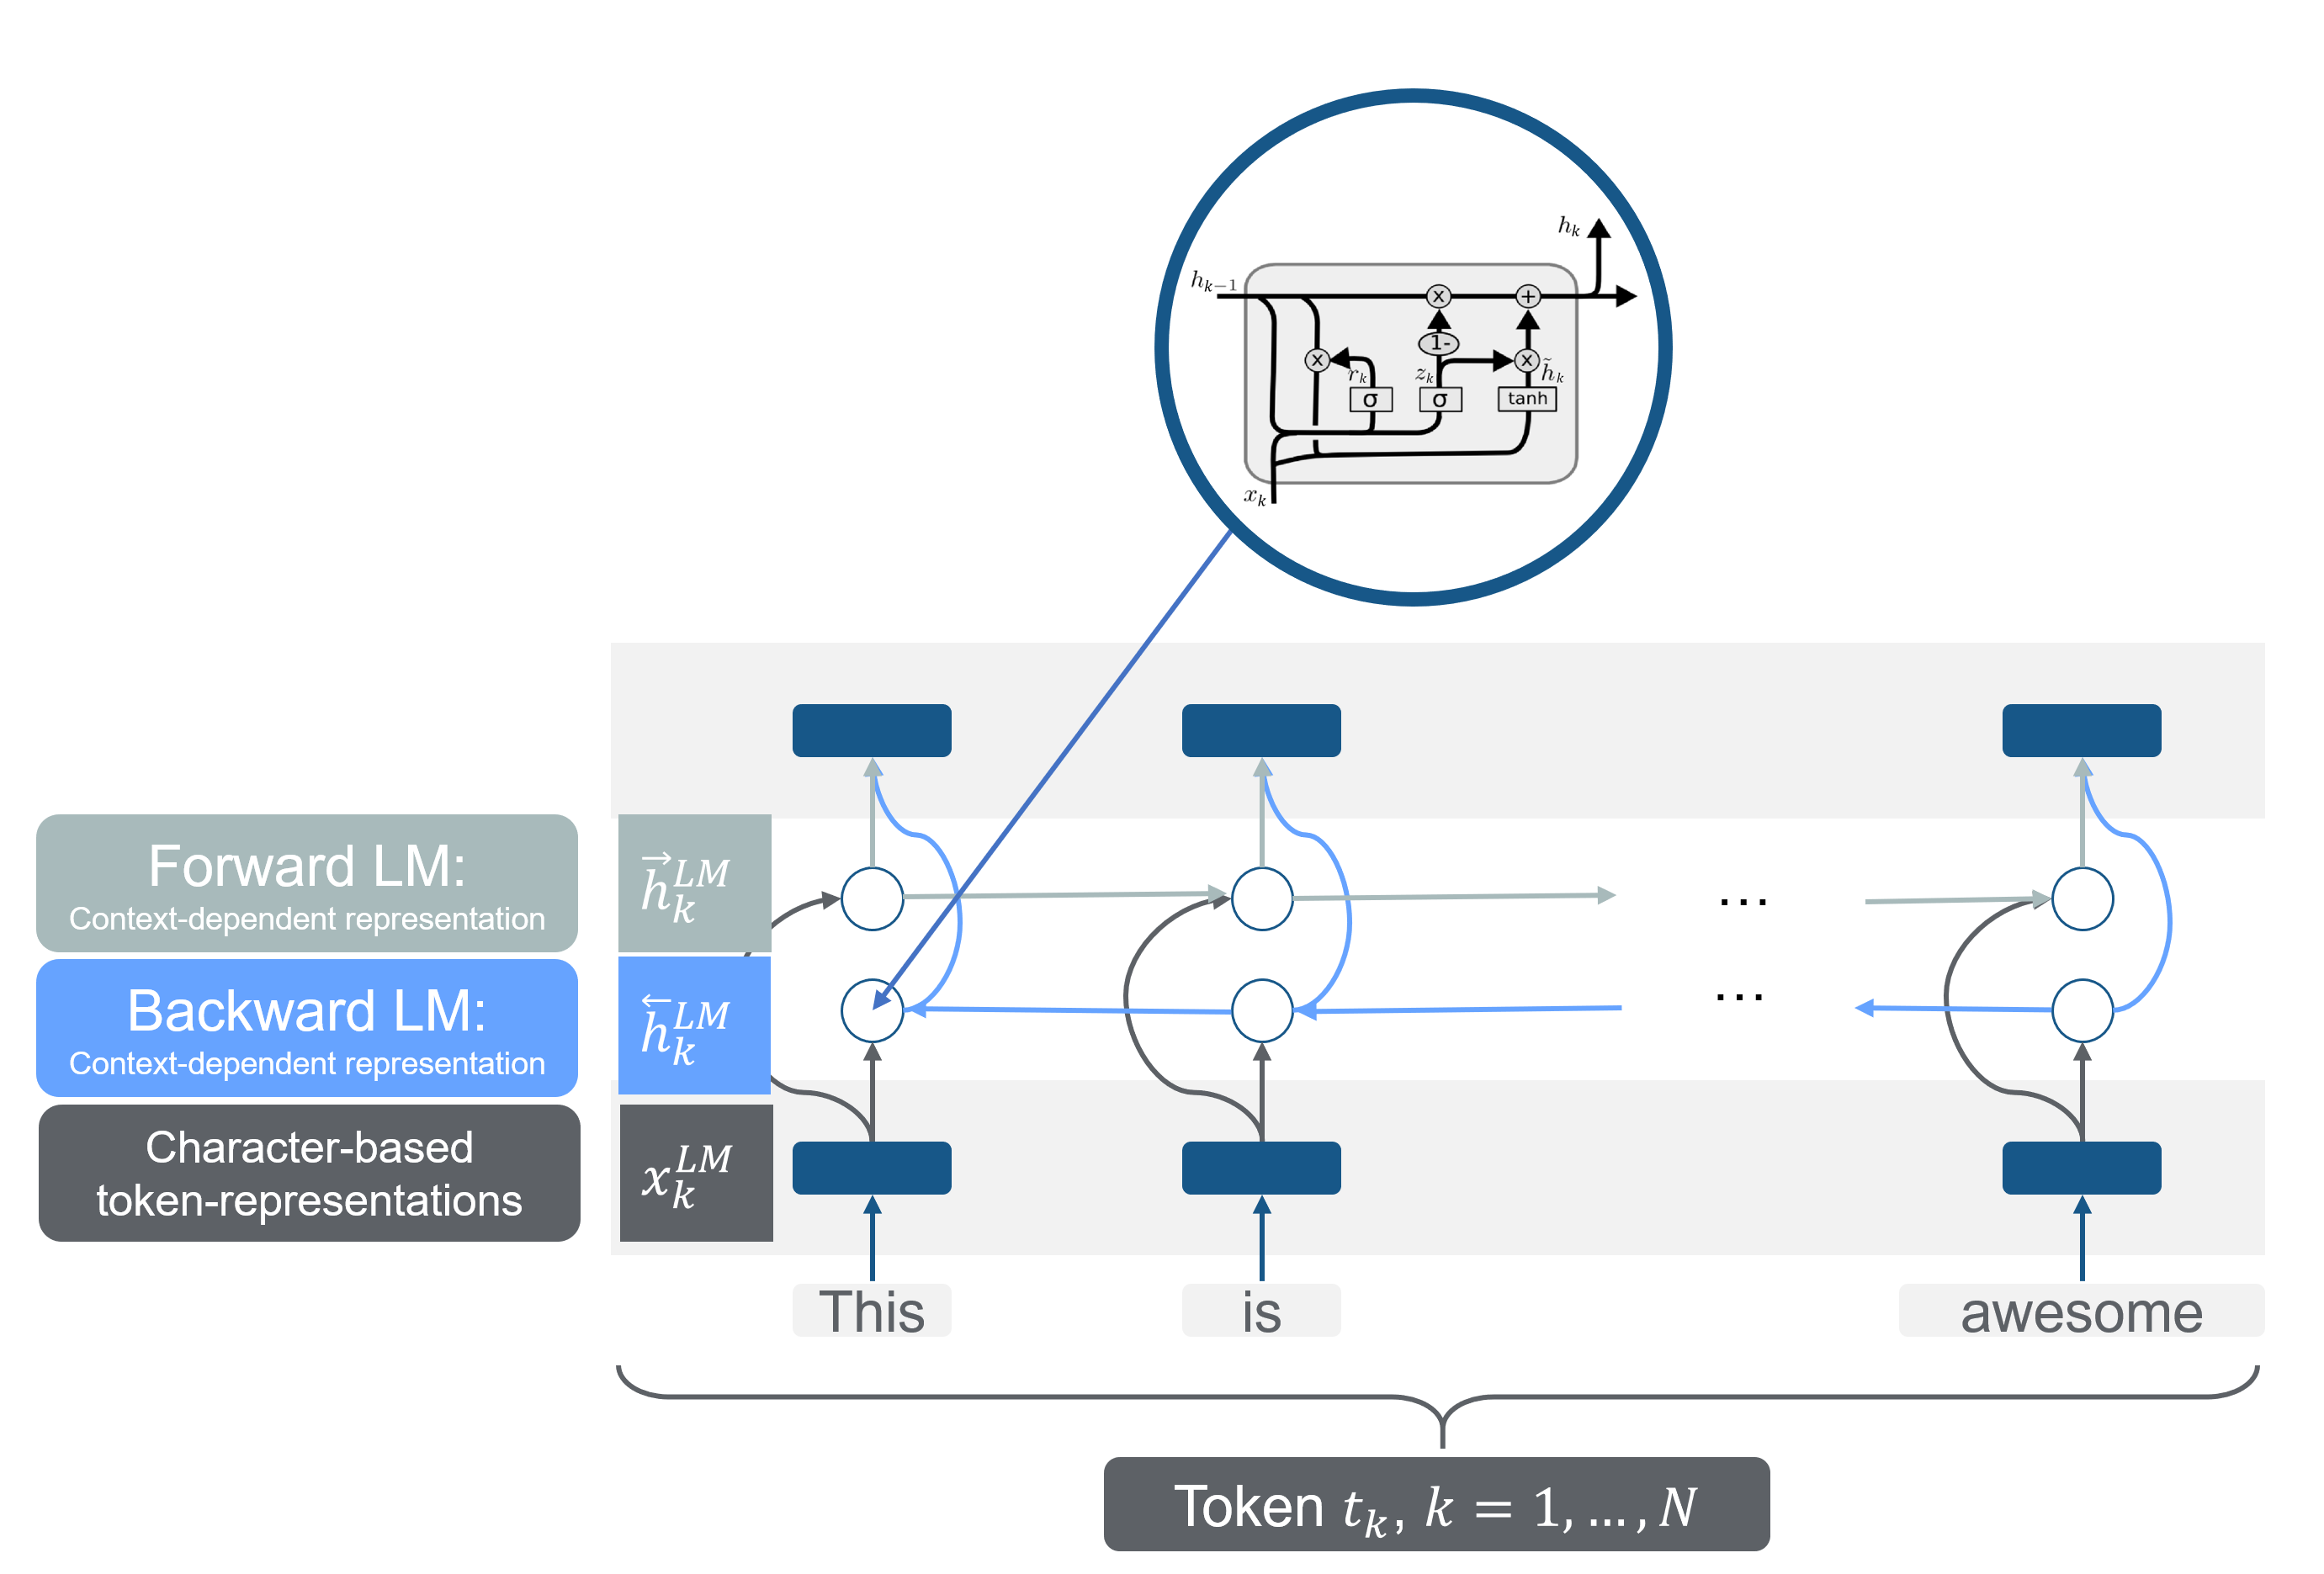
\includegraphics[width = 10cm]{figure/elmo-pretrained-bilm}\\ 
		\footnotesize{Source:} \href{https://compstat-lmu.github.io/seminar_nlp_ss20/transfer-learning-for-nlp-i.html}{\footnotesize \it Carolin Becker}
	\end{figure}
\end{frame}



\begin{frame}{ELMo -- Graphical representation}
	\begin{figure}
		\centering
		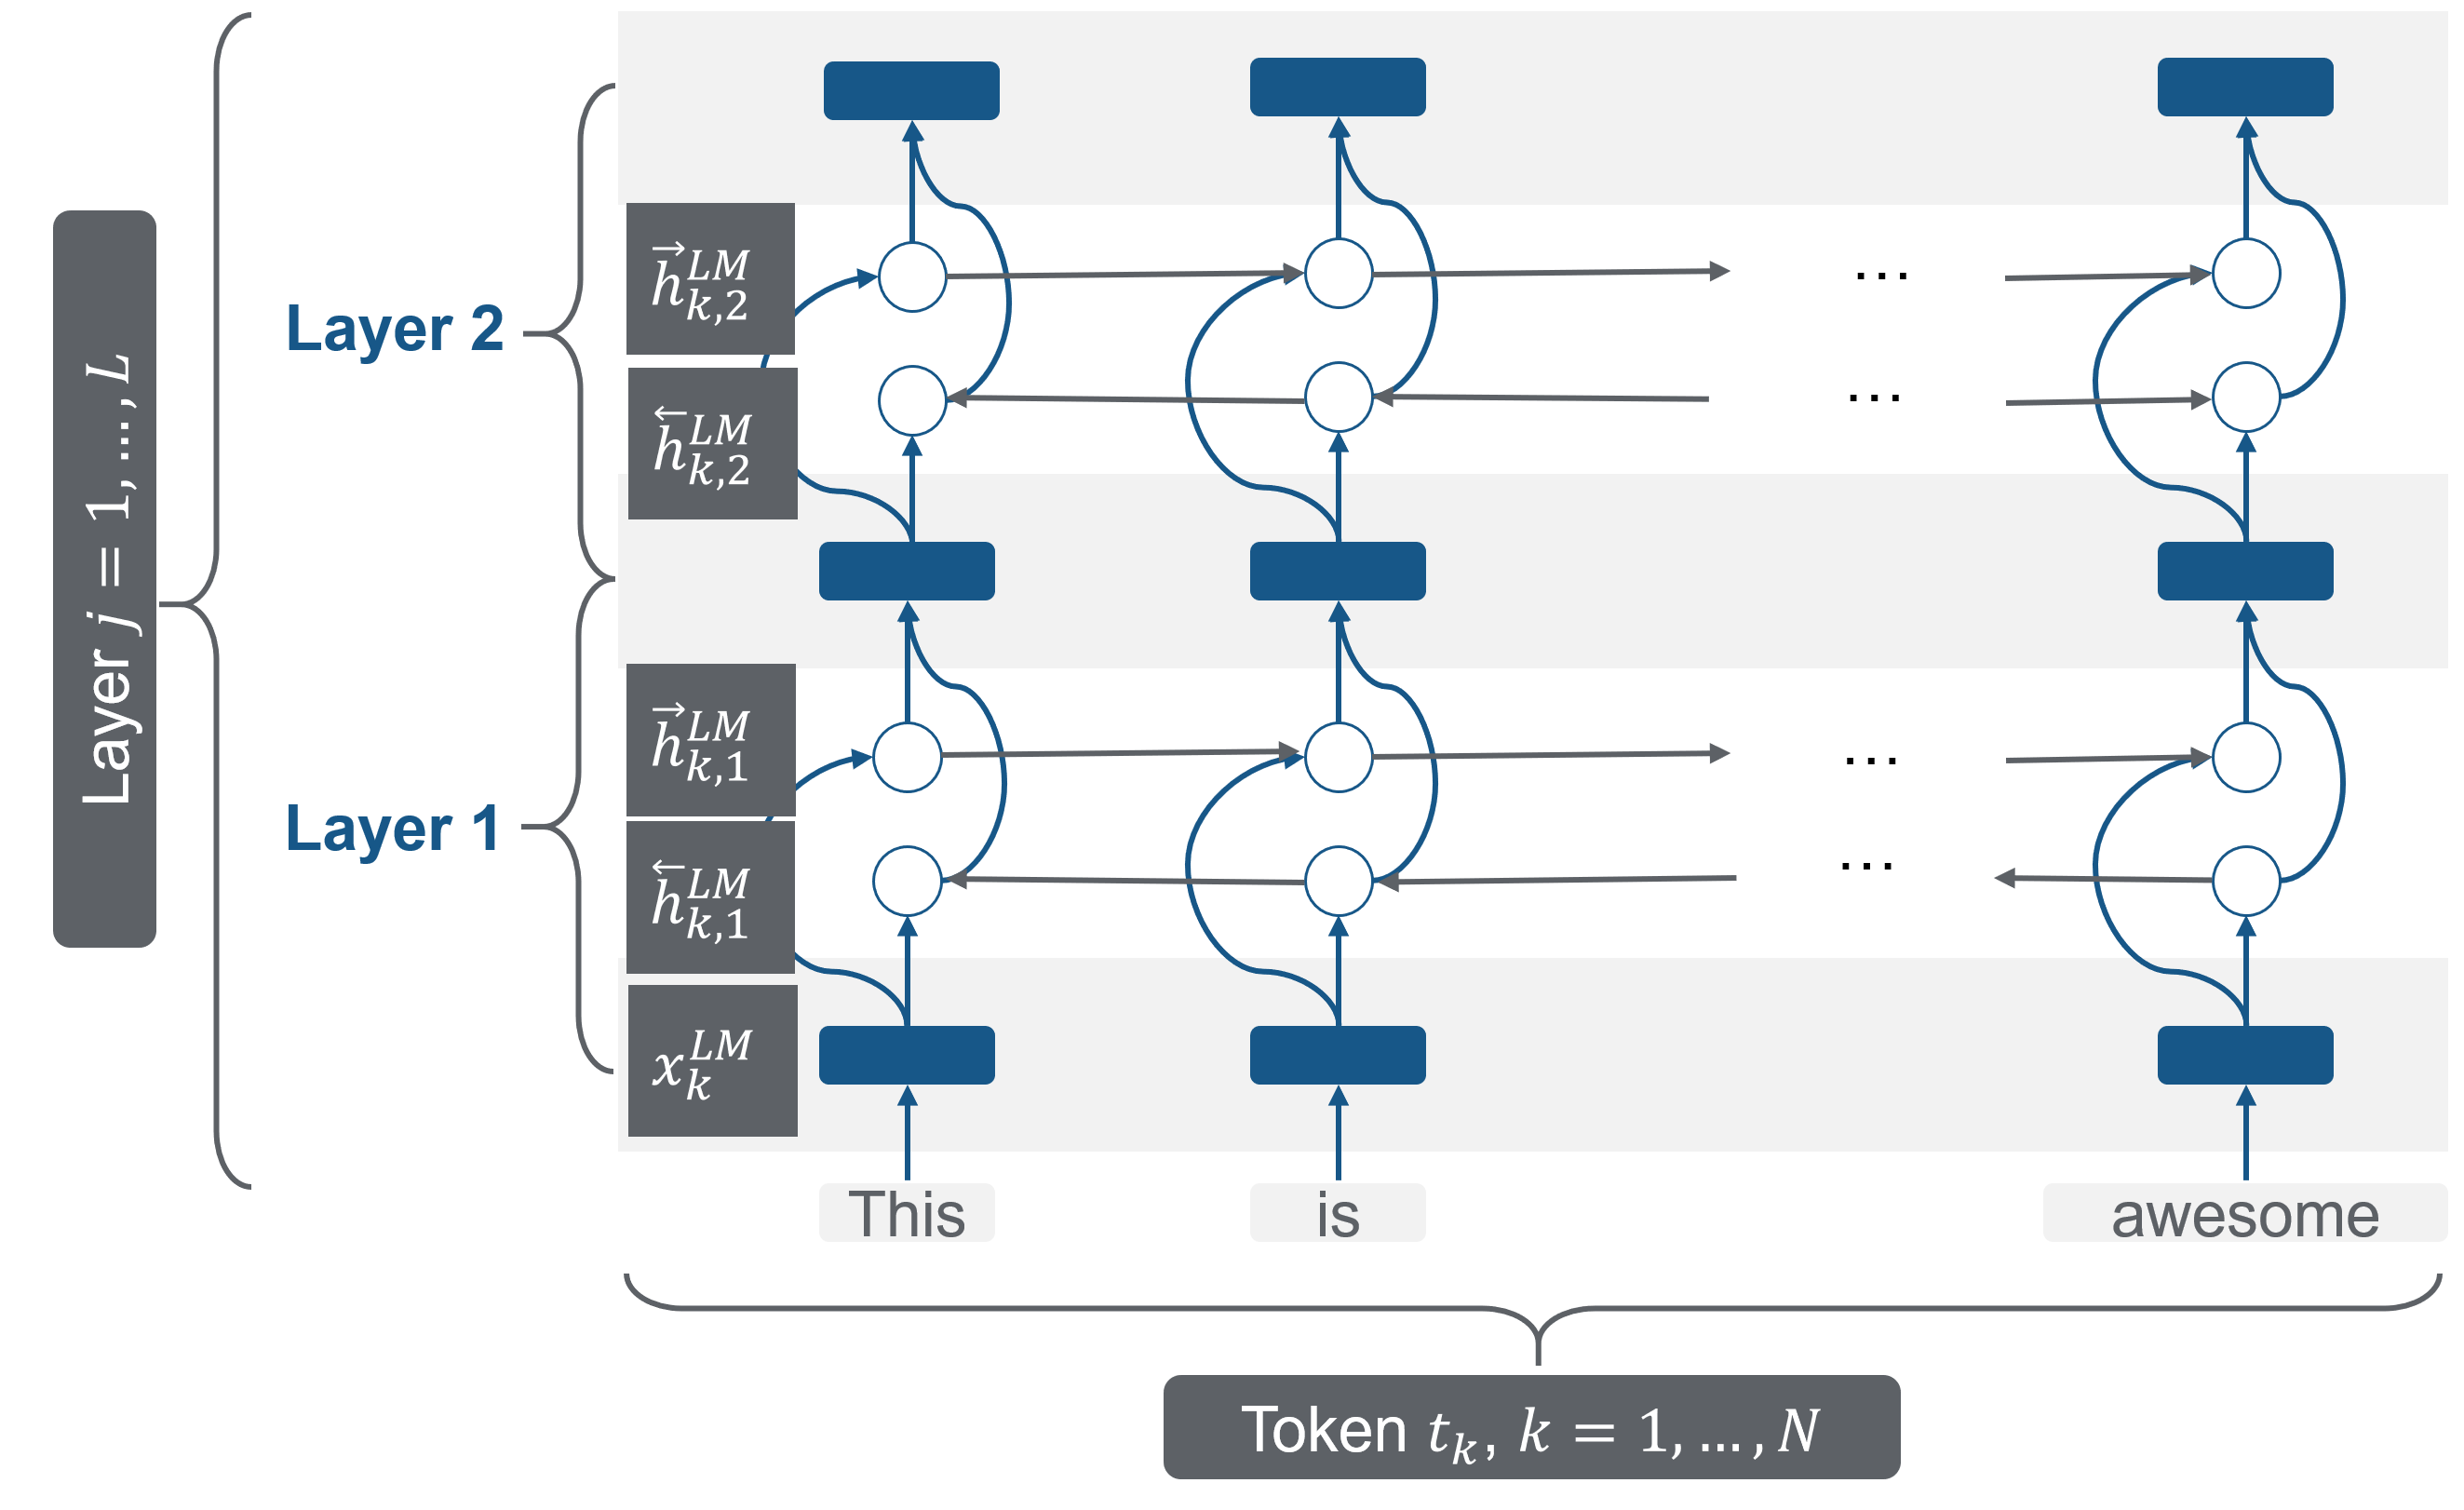
\includegraphics[width = 10cm]{figure/elmo-pretrained-bilm-2}\\ 
		\footnotesize{Source:} \href{https://compstat-lmu.github.io/seminar_nlp_ss20/transfer-learning-for-nlp-i.html}{\footnotesize \it Carolin Becker}
	\end{figure}
\end{frame}



\begin{frame}{ELMo -- Task Adaption}

	\textbf{Including ELMo in downstream tasks:}

	\begin{itemize}
		\item Calculate task-specific weights of all five representations:
					$$\mathbf{E} \mathbf{L} \mathbf{M} \mathbf{o}_{k}^{t a s k}=E\left(R_{k} ; \Theta^{t a s k}\right)=\gamma^{t a s k} \sum_{j=0}^{L} s_{j}^{t a s k} \mathbf{h}_{k, j}^{L M},$$
					where the $\mathbf{h}_{k, j}^{L M}$ are \textbf{not trainable} anymore.
		\item Trainable parameters during the adaption:
			\begin{itemize}
				\item $s_{j}^{t a s k}$ are trainable (softmax-normalized) weights
				\item $\gamma^{t a s k}$ is a trainable scaling parameter
			\end{itemize}
	\end{itemize}

	\textbf{Advantages over context free-embeddings:}

	\begin{itemize}
		\item Task-specific model has access to \textit{multiple} representations of each token
		\item Model learns to which degree to use the different representations depending on the task at hand
	\end{itemize}
\end{frame}



\begin{frame}{ELMo -- Task Adaption}
	\begin{figure}
		\centering
		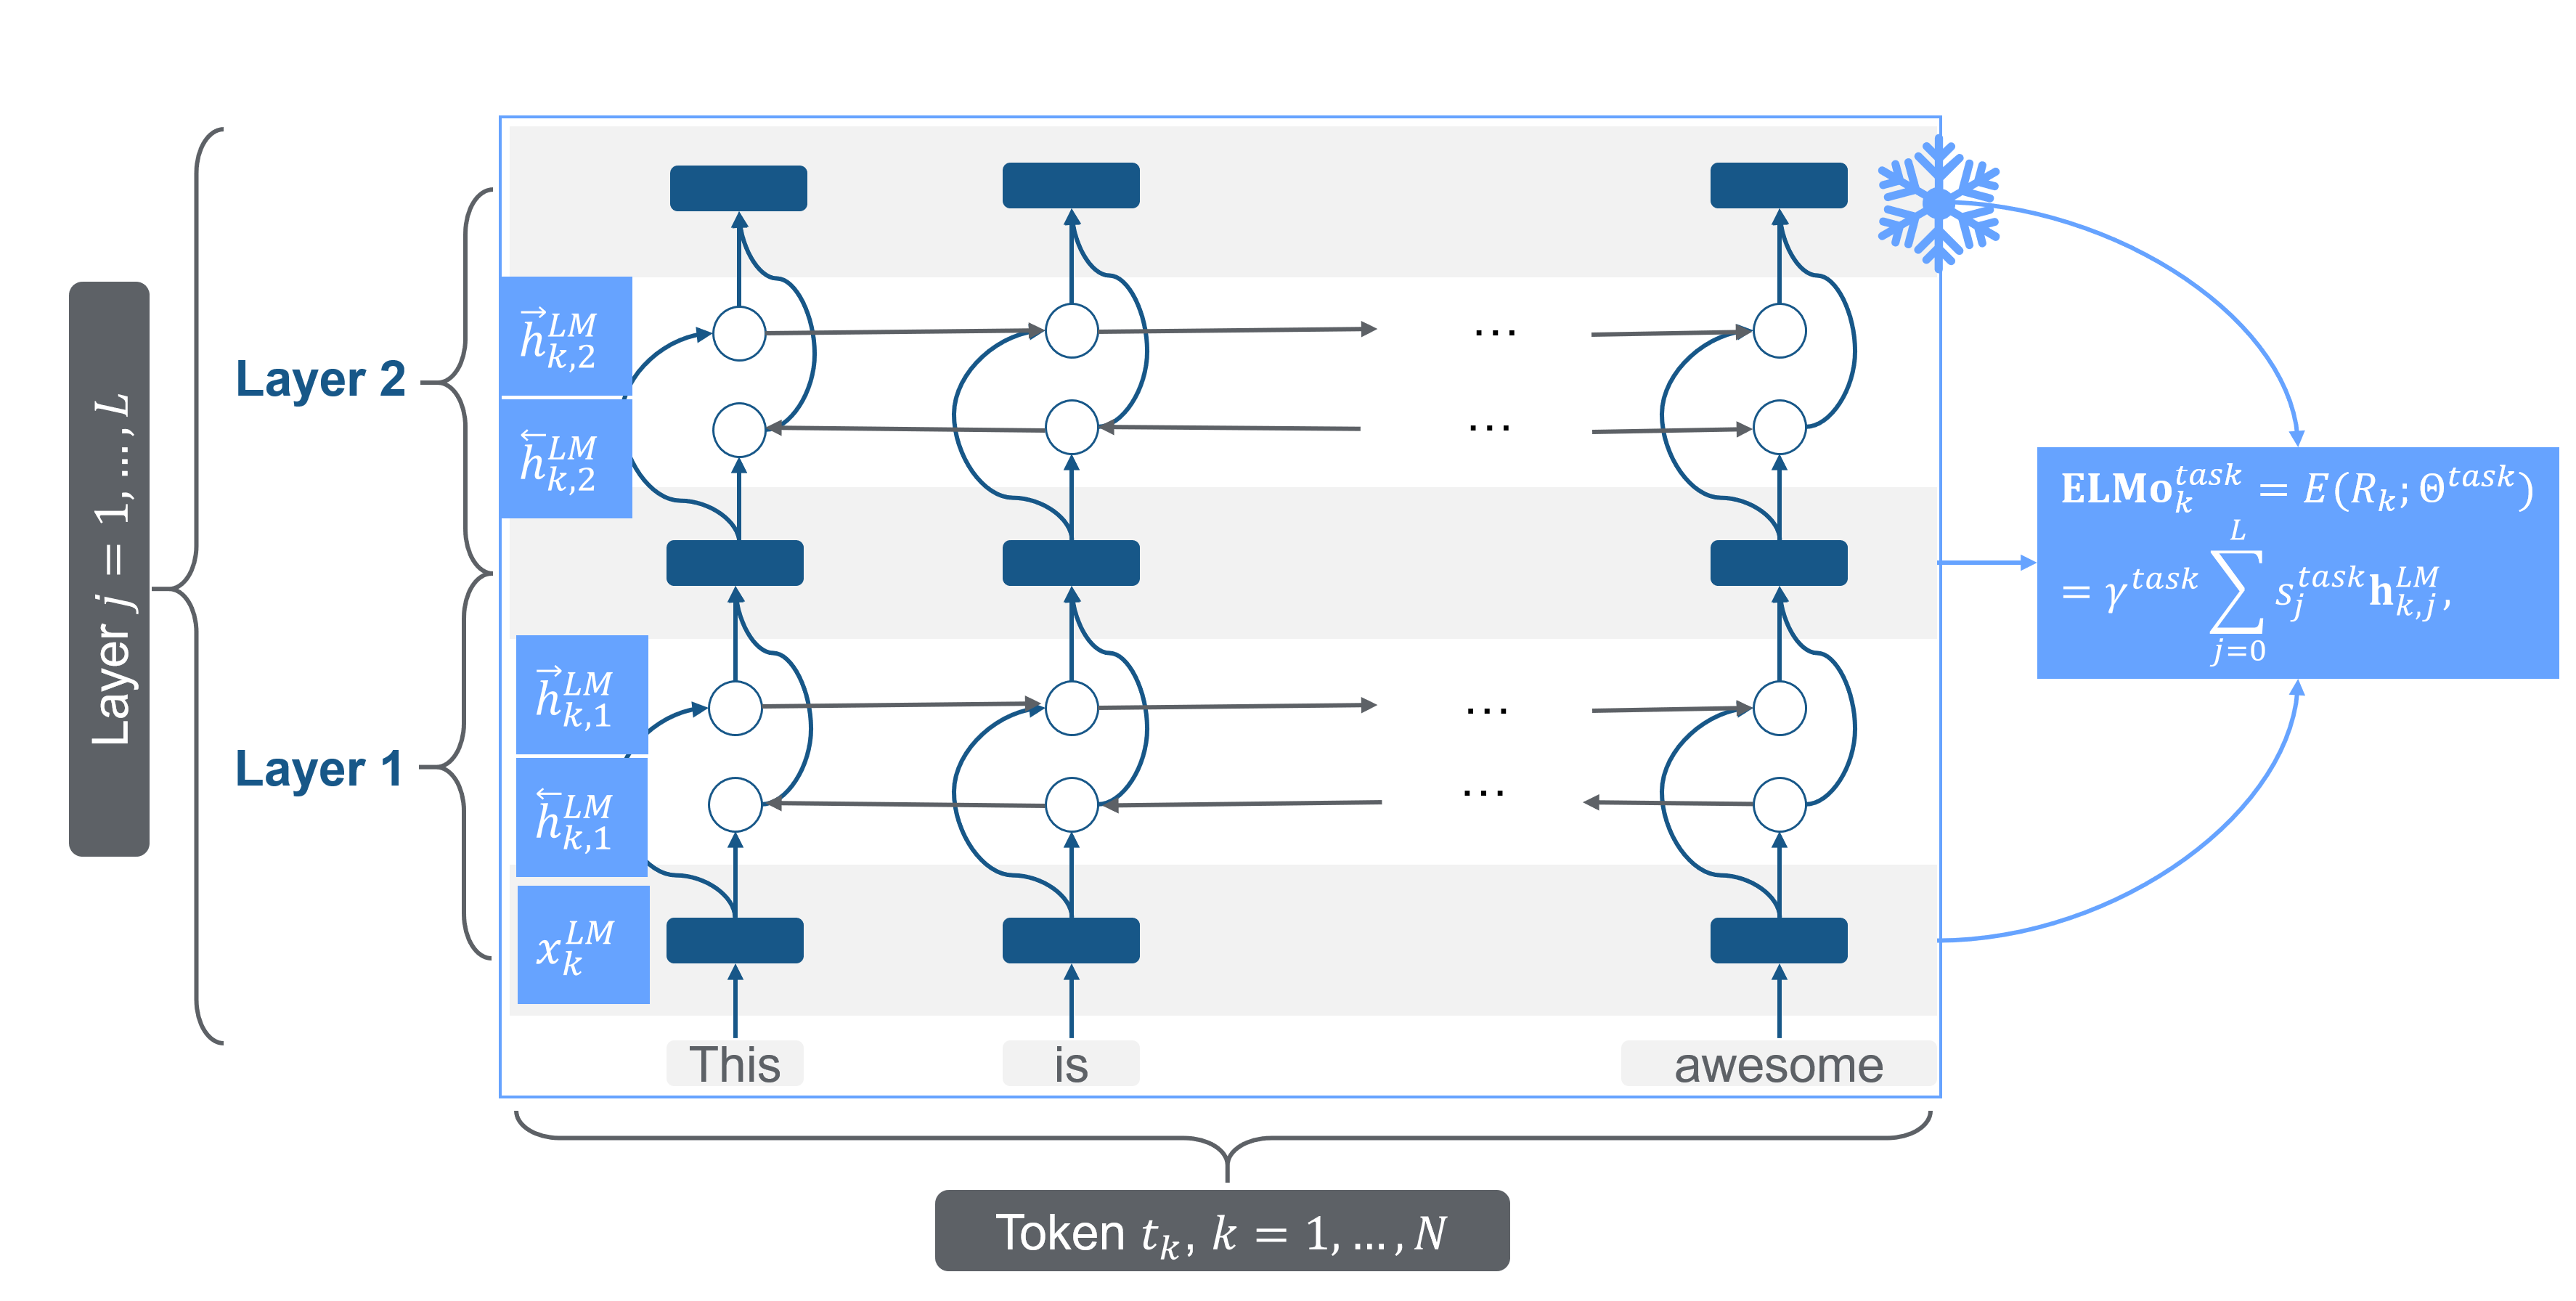
\includegraphics[width = 12cm]{figure/elmo-adaption}\\ 
		\footnotesize{Source:} \href{https://compstat-lmu.github.io/seminar_nlp_ss20/transfer-learning-for-nlp-i.html}{\footnotesize \it Carolin Becker}
	\end{figure}
\end{frame}



\begin{frame}{Fine-tuning approach}

	\textbf{Shortcomings of ELMo:}

	\begin{itemize}
		\item Pre-trained on a general domain corpus, embeddings are not adapted to the domain/task at hand
		\item Sequential nature of LSTMs:
			\begin{itemize}
				\item Not fully parallelizable (compared to Transformers)
				\item Fail to capture long-range dependency during contextualization
			\end{itemize}
	\end{itemize}

	\vspace{.3cm}
	
	\textbf{Alleviations/Alternatives:}

	\begin{itemize}
		\item ULMFiT \href{https://www.aclweb.org/anthology/P18-1031.pdf}{\beamergotobutton{Howard and Ruder, 2018}} is a uni-directional LSTM which is fine-tuned as a whole model on data from the target domain/task.
		\item GPT \href{https://s3-us-west-2.amazonaws.com/openai-assets/research-covers/language-unsupervised/language_understanding_paper.pdf}{\beamergotobutton{Radford et al., 2018}} is a Transformer (decoder) which is fine-tuned as a whole model on data from the target domain/task.
	\end{itemize}
\end{frame}



\begin{frame}{ULMFiT \href{https://www.aclweb.org/anthology/P18-1031.pdf}{\beamergotobutton{Howard and Ruder, 2018}}}
	\begin{figure}
		\centering
		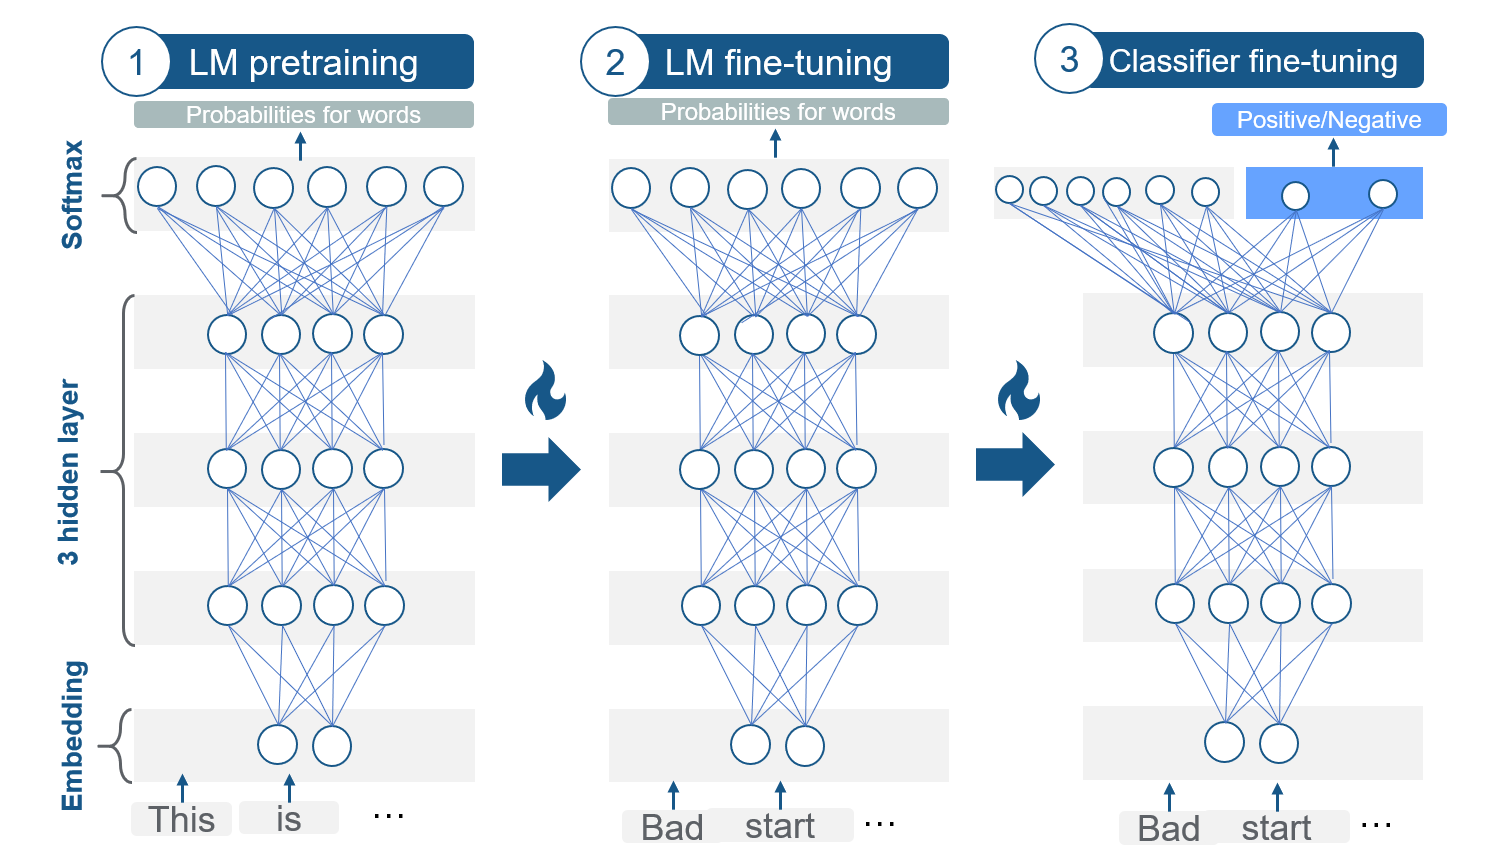
\includegraphics[width = 12cm]{figure/ulmfit-overview-new}\\ 
		\footnotesize{Source:} \href{https://compstat-lmu.github.io/seminar_nlp_ss20/transfer-learning-for-nlp-i.html}{\footnotesize \it Carolin Becker}
	\end{figure}
\end{frame}



\begin{frame}{ULMFiT -- Architectural Details}

	\begin{itemize}
		\item AWD-LSTMs \href{https://arxiv.org/pdf/1708.02182.pdf}{\beamergotobutton{Merity et al., 2017}} as backbone of the architecture
			\begin{itemize}
				\item DropConnect \href{http://proceedings.mlr.press/v28/wan13.pdf}{\beamergotobutton{Wan et al., 2013}}
				\item Averaged stochastic gradient descent (ASGD) for optimiziation
			\end{itemize}
		\item Embedding layer + three LSTM layers + Softmax Layer
		\item \textbf{LM fine-tuning:}
			\begin{itemize}
				\item Discriminative fine-tuning 
			\end{itemize}
		\item \textbf{Classifier fine-tuning:}
			\begin{itemize}
				\item Concat Pooling
				\item Gradual unfreezing
			\end{itemize}
	\end{itemize}
\end{frame}



\begin{frame}{GPT \href{https://s3-us-west-2.amazonaws.com/openai-assets/research-covers/language-unsupervised/language_understanding_paper.pdf}{\beamergotobutton{Radford et al., 2018}}}
	\begin{figure}
		\centering
		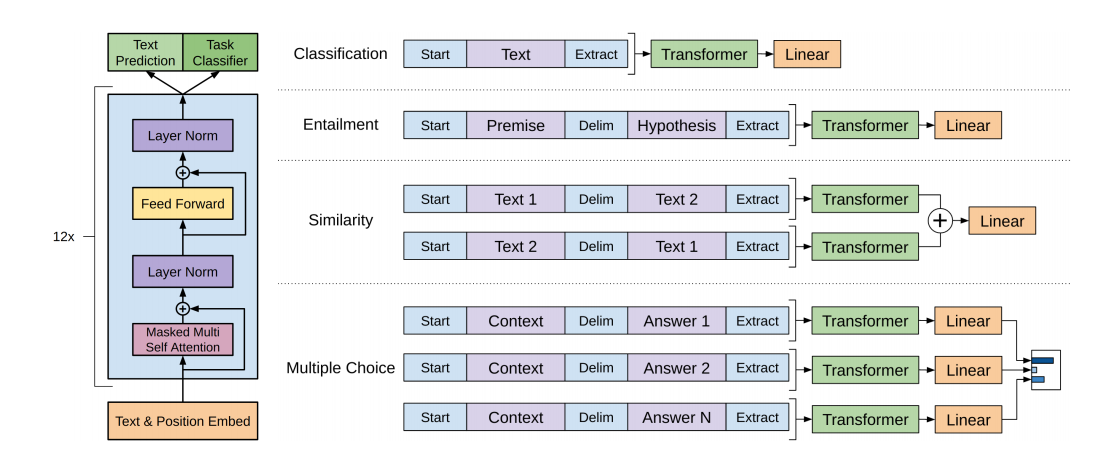
\includegraphics[width = 12cm]{figure/gpt}\\ 
		\footnotesize{Source:} \href{https://s3-us-west-2.amazonaws.com/openai-assets/research-covers/language-unsupervised/language_understanding_paper.pdf}{\footnotesize \it Radford et al., 2018}
	\end{figure}
\end{frame}



\begin{frame}{GPT -- Architectural Details}
	\begin{itemize}
		\item Transformer decoder as backbone of the architecture
			\begin{itemize}
				\item 12-layer-decoder with masked attention heads
				\item 40k BPE vocabulary
				\item Learned positional embeddings (compared to sinusoidal versions)
			\end{itemize}
		\item \textbf{Fine-tuning:}
			\begin{itemize}
				\item Linear output layer with softmax activation on top
				\item Auxiliary language modeling objective during fine-tuning\\
							$\rightarrow$ Improves generalization\\
							$\rightarrow$ Accelerates convegence
				\item Task-specific input transformations (see previous slide)
			\end{itemize}
	\end{itemize}
\end{frame}



\begin{frame}{GPT -- SOTA results}

	\textbf{Performance on different benchmarks:}

	\begin{figure}
		\centering
		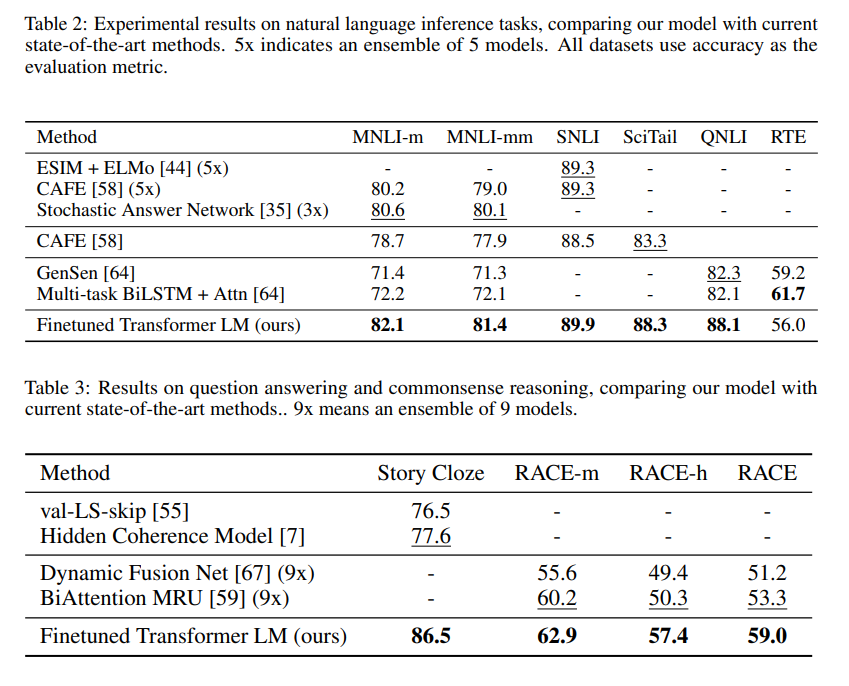
\includegraphics[width = 8cm]{figure/gpt-sota.png}\\ 
		\footnotesize{Source:} \href{https://s3-us-west-2.amazonaws.com/openai-assets/research-covers/language-unsupervised/language_understanding_paper.pdf}{\footnotesize Radford et al. (2018)}
	\end{figure}
\end{frame}



\begin{frame}{Pre-training objectives}

	\textbf{Self-Supervision:}

	\begin{itemize}
		\item Special case of unsupervised learning
		\item Labels are generated from the data itself
	\end{itemize}
	
	\vspace{.3cm}
	
	\textbf{Self-supervised objectives:}
	
	\begin{itemize}
		\item Skip-gram objective (cf. word2vec \href{https://arxiv.org/pdf/1301.3781.pdf}{\beamergotobutton{Mikolov et al. (2013a)}})
		\item Language modeling objective (cf. \href{http://www.jmlr.org/papers/volume3/bengio03a/bengio03a.pdf}{\beamergotobutton{Bengio et al. (2003)}})
		\item \textit{Masked language modeling (MLM)} objective (cf. chapter 10)\\
					$\rightarrow$ Replace words by a \texttt{[MASK]} token and train the model to predict
		\item \textit{Permutation language modeling (PLM)} objective (cf. chapter 11)\\
					$\rightarrow$ Autoregressive objective of XLNet
		\item \textit{Replaced token detection} objective (cf. chapter 11)\\
					$\rightarrow$ Requires two models: One performing MLM \& the second model to discriminate between actual and the predicted tokens
	\end{itemize}
\end{frame}



\begin{frame}{Pre-training resources}

	\textbf{Commonly used (large-scale) data sets for pre-training}

	\begin{itemize}
		\item English Wikipedia
		\item 1B Word Benchmark \href{https://arxiv.org/pdf/1312.3005.pdf}{\beamergotobutton{Chelba et al. (2013)}}
		\item BooksCorpus \href{https://www.cv-foundation.org/openaccess/content_iccv_2015/papers/Zhu_Aligning_Books_and_ICCV_2015_paper.pdf}{\beamergotobutton{Zhu et al. (2015)}}
		\item Wikitext-103 \href{https://academictorrents.com/details/a4fee5547056c845e31ab952598f43b42333183c}{\beamergotobutton{Merity et al. (2016)}}
		\item CommonCrawl \href{https://commoncrawl.org/}{\beamergotobutton{https://commoncrawl.org/}}
	\end{itemize}
	
	\vspace{.3cm}

	\textbf{Non-exhaustive list; tbc in the following chapters}
\end{frame}



\begin{frame}{Transfer Learning in Computer Vision}

	\textbf{ImageNet:} \href{https://www.researchgate.net/profile/Li_Jia_Li/publication/221361415_ImageNet_a_Large-Scale_Hierarchical_Image_Database/links/00b495388120dbc339000000/ImageNet-a-Large-Scale-Hierarchical-Image-Database.pdf}{\beamergotobutton{Deng et al., 2009}}

	\begin{itemize}
		\item Large-scale data set ($\approx$ 50 million labeled images)
		\item Hierarchical data set structured in synsets
		\item "\textit{Diverse coverage of the image world.}" (Deng et al., 2009)
	\end{itemize}
	
	\vspace{.3cm}
	
	\textbf{How it changed learning:}
	
	\begin{itemize}
		\item Quasi-standard to use a model pre-trained on ImageNet
		\item Achieved SOTA results in various computer vision tasks
		\item Enable the use of large models to small (labeled) data sets
	\end{itemize}
\end{frame}



\begin{frame}{Summary \& Outlook}

	\textbf{Pros:}

	\begin{itemize}
		\item New and deep architectures enable better representation learning 
		\item Leverage favorable properties of language to create self-supervised tasks
		\item Use ubiquitous large amounts of unlabeled data available on the web
	\end{itemize}
	
	\vspace{.3cm}
	
	\textbf{Cons:}
	
	\begin{itemize}
		\item Pre-Training \textit{extremely} costly
		\item Models will have up to over billions parameters 
		\item Only works well for high-resource languages
	\end{itemize}
\end{frame}



\begin{frame}{Further reading}

	\begin{itemize}
		\item \href{https://thegradient.pub/nlp-imagenet/}{\textit{NLP's ImageNet moment has arrived}}
		\item Sebastian Ruder's PhD thesis: \href{https://ruder.io/thesis/}{\beamergotobutton{Ruder, 2019}}
	\end{itemize}
	
\end{frame}



\end{document}